\documentclass[a4paper,12pt]{report}

\usepackage{cmap}
\usepackage[T2A]{fontenc}
\usepackage[utf8]{inputenc}
\usepackage[russian]{babel}
\usepackage{amsmath,amsfonts,amssymb}
\usepackage{graphicx}
\usepackage{sidecap}
\usepackage{wrapfig}


\begin{document} 

\begin{titlepage} 

\begin{center} 

\large Федеральное государственное автономное образовательное учреждение высшего образования «Санкт-Петербургский государственный электротехнический университет «ЛЭТИ» им. В.И. Ульянова (Ленина)»

кафедра теоретических основ электротехники\\[5cm] 

\huge ОТЧЕТ\\ по лабораторной работе № 3\\[0.5cm] 
\large <<ИССЛЕДОВАНИЕ СВОБОДНЫХ ПРОЦЕССОВ В ЭЛЕКТРИЧЕСКИХ ЦЕПЯХ>>\\[3.7cm]

\begin{minipage}{1\textwidth} 
    \begin{flushleft} 
        \emph{Авторы:} Стукен В.А. , Зиновьев М.Д\\
        \emph{Группа:} 2307\\
        \emph{Факультет:} ФКТИ\\
        \emph{Преподаватель:} Зубарев А.В
    \end{flushleft} 
\end{minipage} 

\vfill 

Санкт-Петербург, 2024\\
{\large \LaTeX} 

\end{center} 

\thispagestyle{empty} 
\end{titlepage} 

\section*{Цель:}
Изучение связи между видом свободного процесса в электрической цепи и расположением ее собственных частот (корней характеристического уравнения) на комплексной плоскости; экспериментальное определение собственных частот и добротности RLC-контура по осциллограммам.

\section*{Экспериментальные исследования}

\begin{flushleft}
    \item\subsection*{Опыт №1 Исследование свободных процессов в цепи первого порядка, $C = 0.02 \cdot 10^{-6} \, \Phi$}
    \item \begin{figure}[h!]
        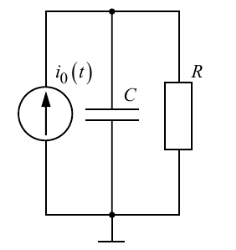
\includegraphics[width=0.5\textwidth]{image.png}
        \label{ris:image1}
        рис. 1 - Схема для опыта №1 
    \end{figure}

     \begin{figure}[h!]
      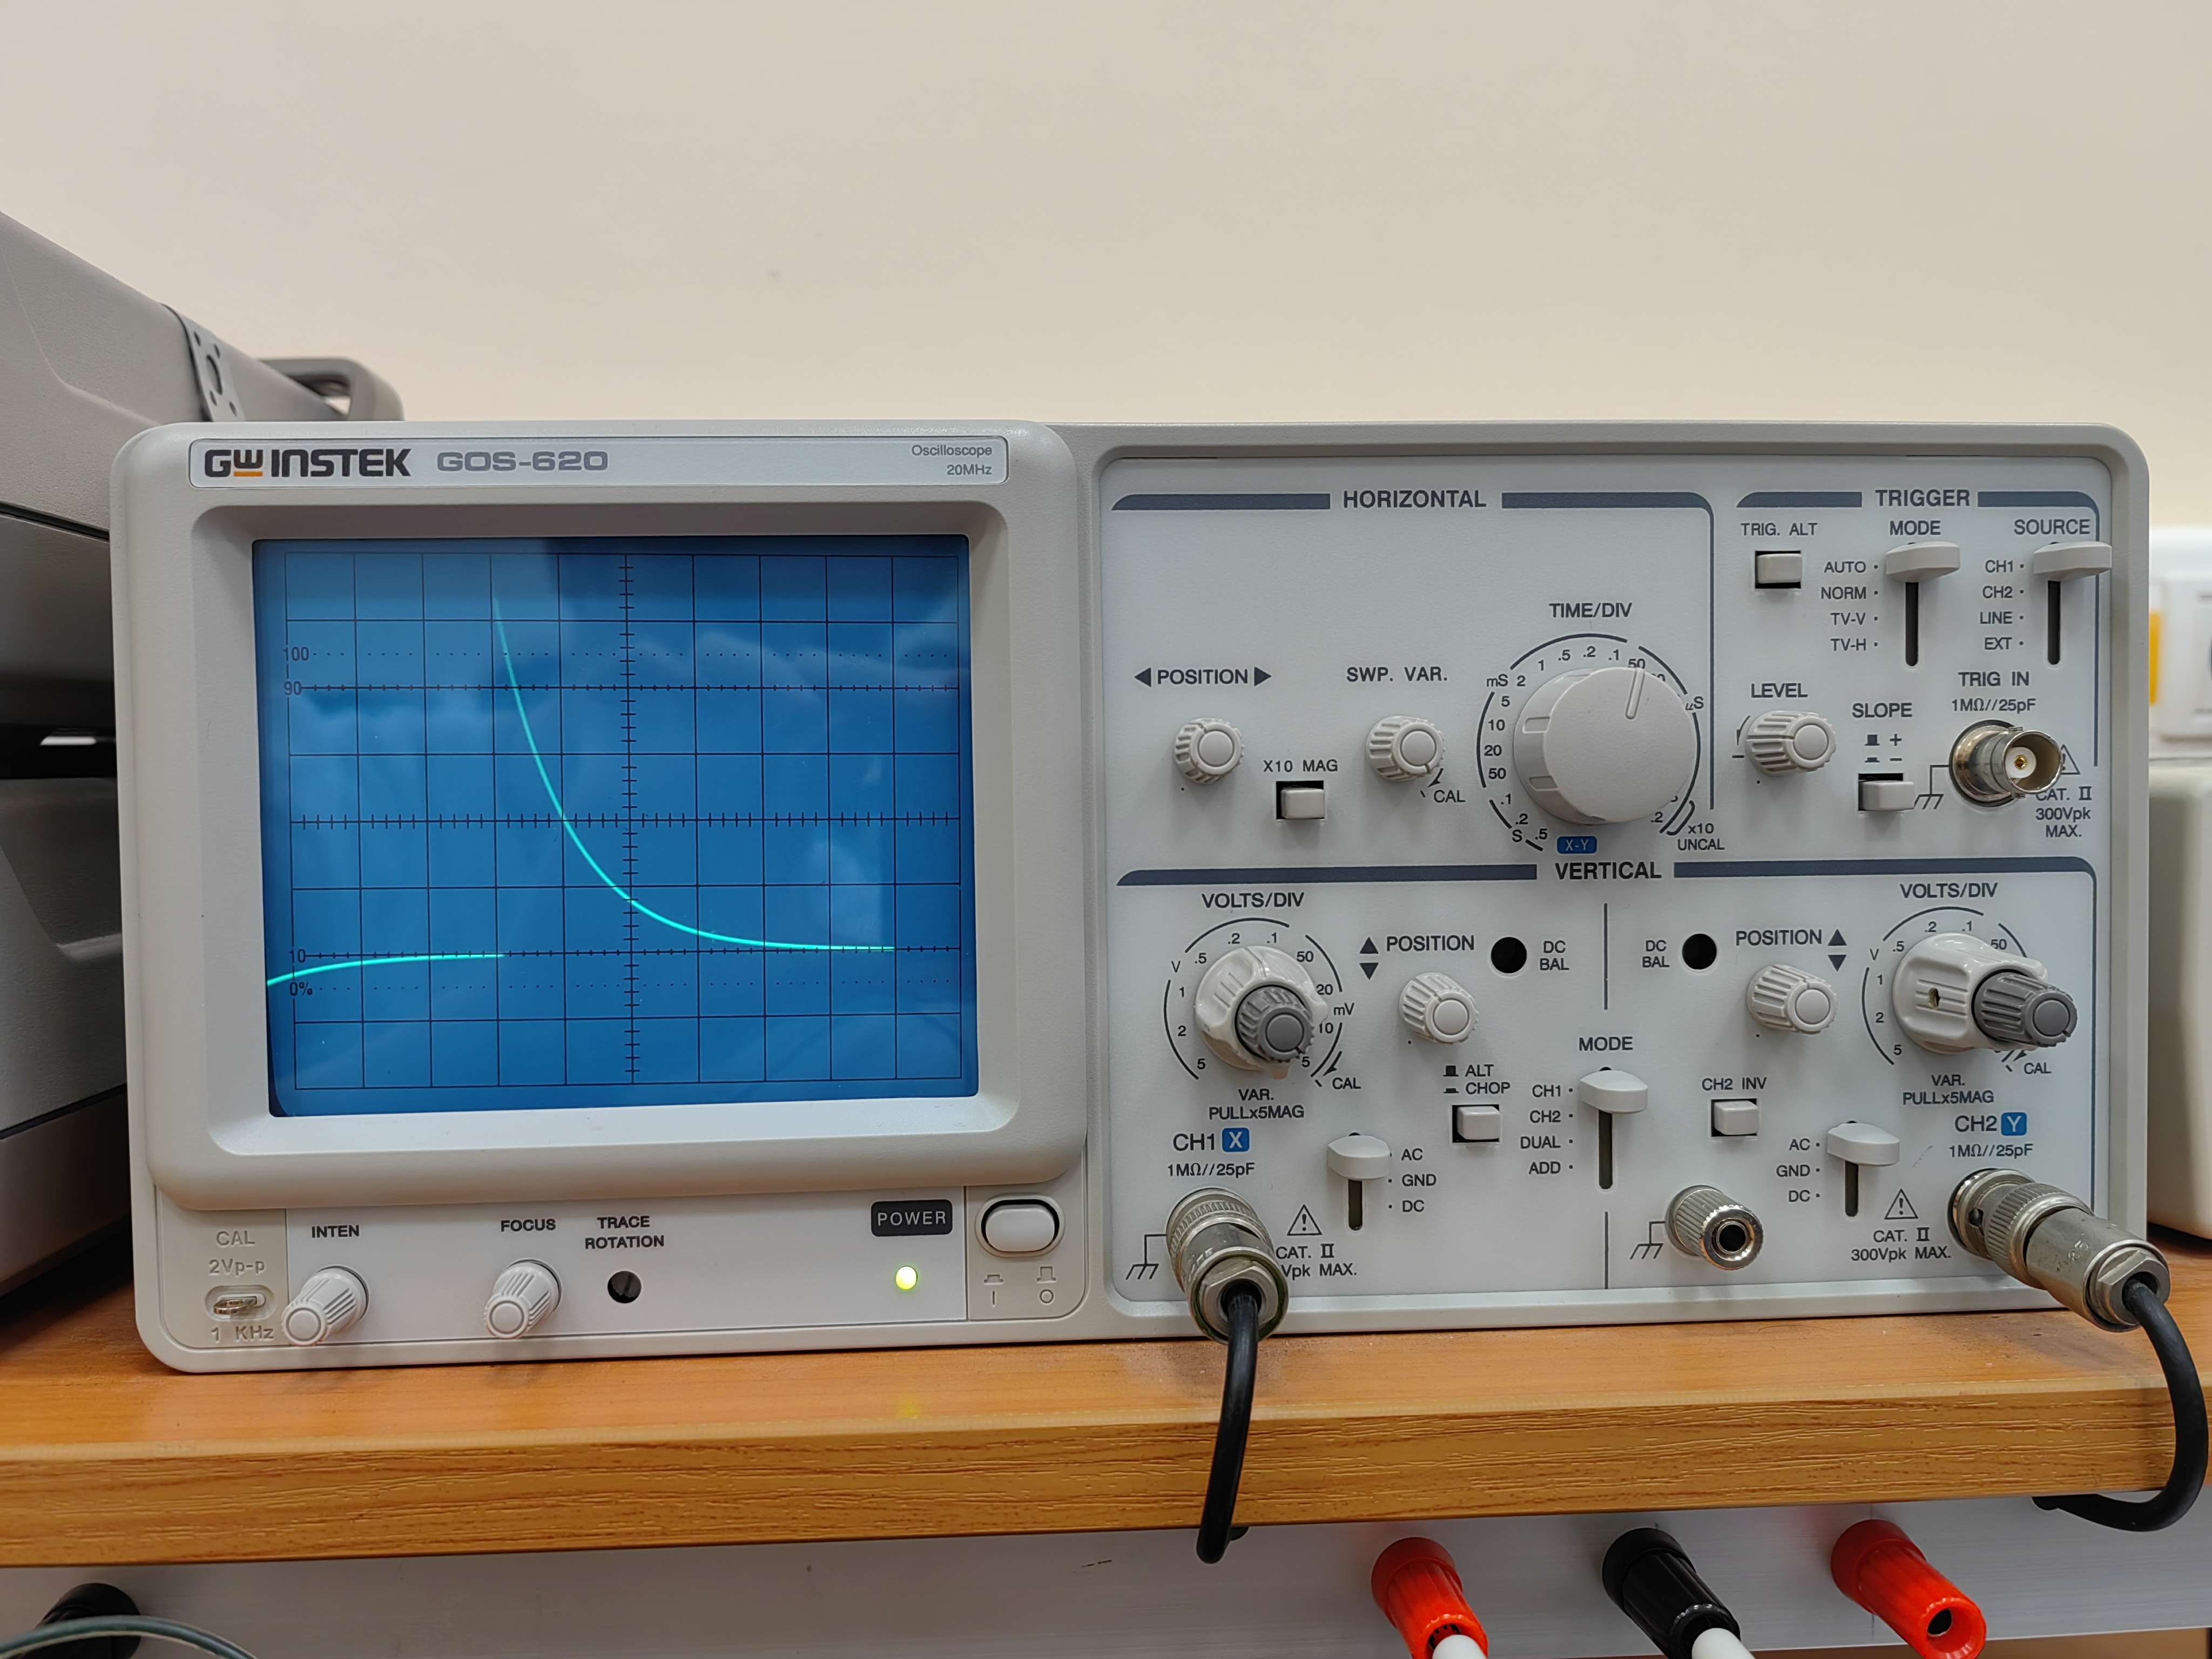
\includegraphics[width=1\textwidth]{graph1.jpg}
      \label{ris:image2}
      рис. 2 - осциллограмма для опыта №1 при R = 5, масштаб $T = .1; V = .2$
  \end{figure}

  \subparagraph*{Вопрос №1 Каким аналитическим выражением описывается осциллографируемый процесс?\\ Осцилографируемый процесс описывается формулой:}
  \[ u(t) = Ae^{p_1t} = Ae^{-at} = Ae^{-t/\tau} \]
  \subparagraph*{Вопрос №2 Соответствует ли найденная собственная частота
  теоретическому расчету?\\ Собственная частота определяется по формуле:}
  \[ p_1 = - \alpha = -\frac{ln(U1/U2)}{\Delta t} \approx \]
  Что соответсвует теоретическому расчету:
  \[ \alpha = - \frac{1}{RC} = \frac{1}{(5\cdot 10^{3})\cdot (0.02\cdot 10^{-6})} = -10000 \]

    \newpage

	\item\subsection*{Опыт №2  Исследование свободного процесса в цепи второго порядка}
	\item
  \begin{figure}[h!]
    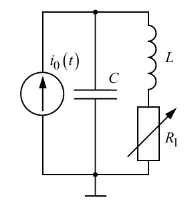
\includegraphics[width=0.5\textwidth]{image2.png}
    \label{ris:image3}
    рис. 3 - Схема для опыта №2 
\end{figure}
\par $C = 0.02 \cdot 10^{-6} \, \Phi$
\par $L = 25 \, mGn$
\newpage
  
\subparagraph*{Найдем собственные частоты при $R_1$ = 0.5 $k\Omega$}

\[ \alpha = \frac{R_1}{2L} = \frac{0.5\cdot 10^3}{2\cdot 25\cdot 10^{-3}} = 10000 \]
\[ \omega_0 = \frac{1}{\sqrt{LC}} = \frac{1}{\sqrt{25\cdot 10^{-3}\cdot 0.02\cdot 10^{-6}}} = 44271 \]
\[ \omega = \sqrt{\omega_0^2 - \alpha^2} = j\cdot 43589 \]
\[ p_{1,2} = -\alpha \pm \sqrt{\omega_0^2 - \alpha^2} = -10000 \pm j\cdot 43589 \]
\begin{figure}[h!]
  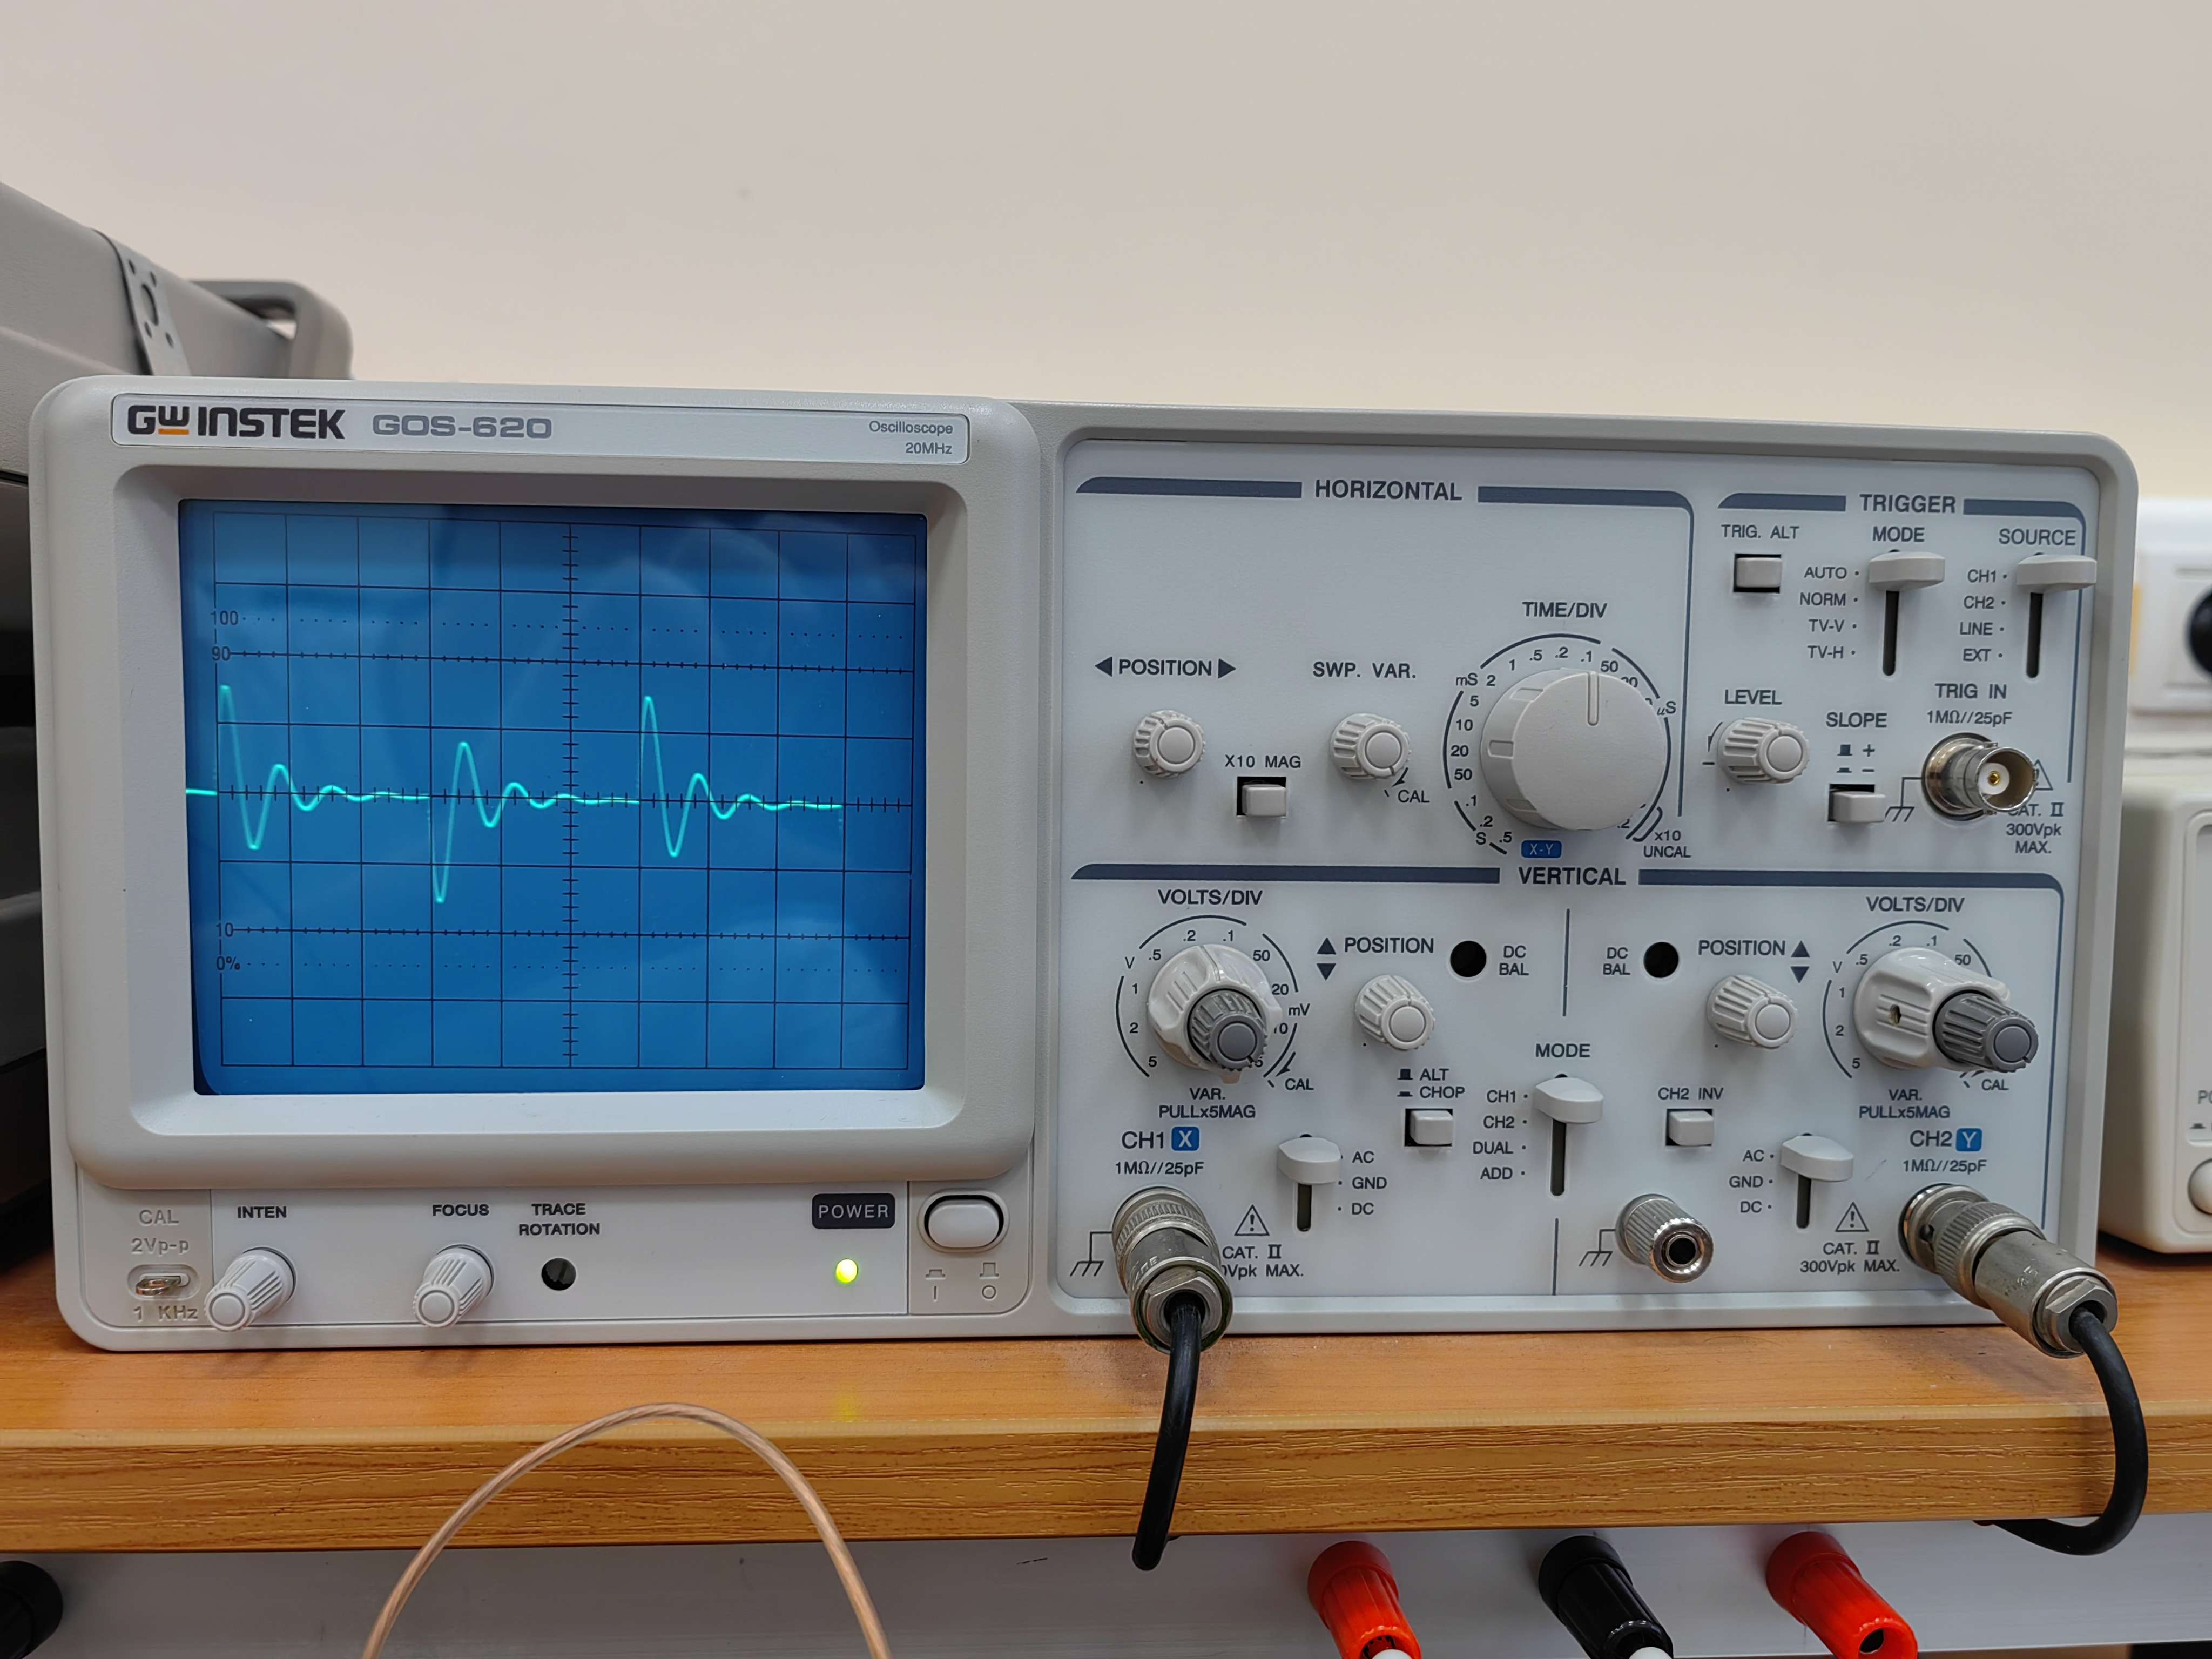
\includegraphics[width=1\textwidth]{graph2.jpg}
  \label{ris:image4}
  рис. 4 - осциллограмма для опыта №2 при R = 0.5, масштаб $T = .2; V = .2$
\end{figure}
\newpage
\subparagraph*{Найдем собственные частоты при $R_2$ = 3 $k\Omega$}

\[ \alpha = \frac{R_2}{2L} = \frac{3\cdot 10^3}{2\cdot 25\cdot 10^{-3}} = 60000 \]
\[ \omega_0 = \frac{1}{\sqrt{LC}} = \frac{1}{\sqrt{25\cdot 10^{-3}\cdot 0.02\cdot 10^{-6}}} =  44721\]
\[ \omega = \sqrt{\omega_0^2 - \alpha^2} = 40000 \]
\[ p_{1,2} = -\alpha \pm \sqrt{\omega_0^2 - \alpha^2} = -60000 \pm  40000 \]
\begin{figure}[h!]
  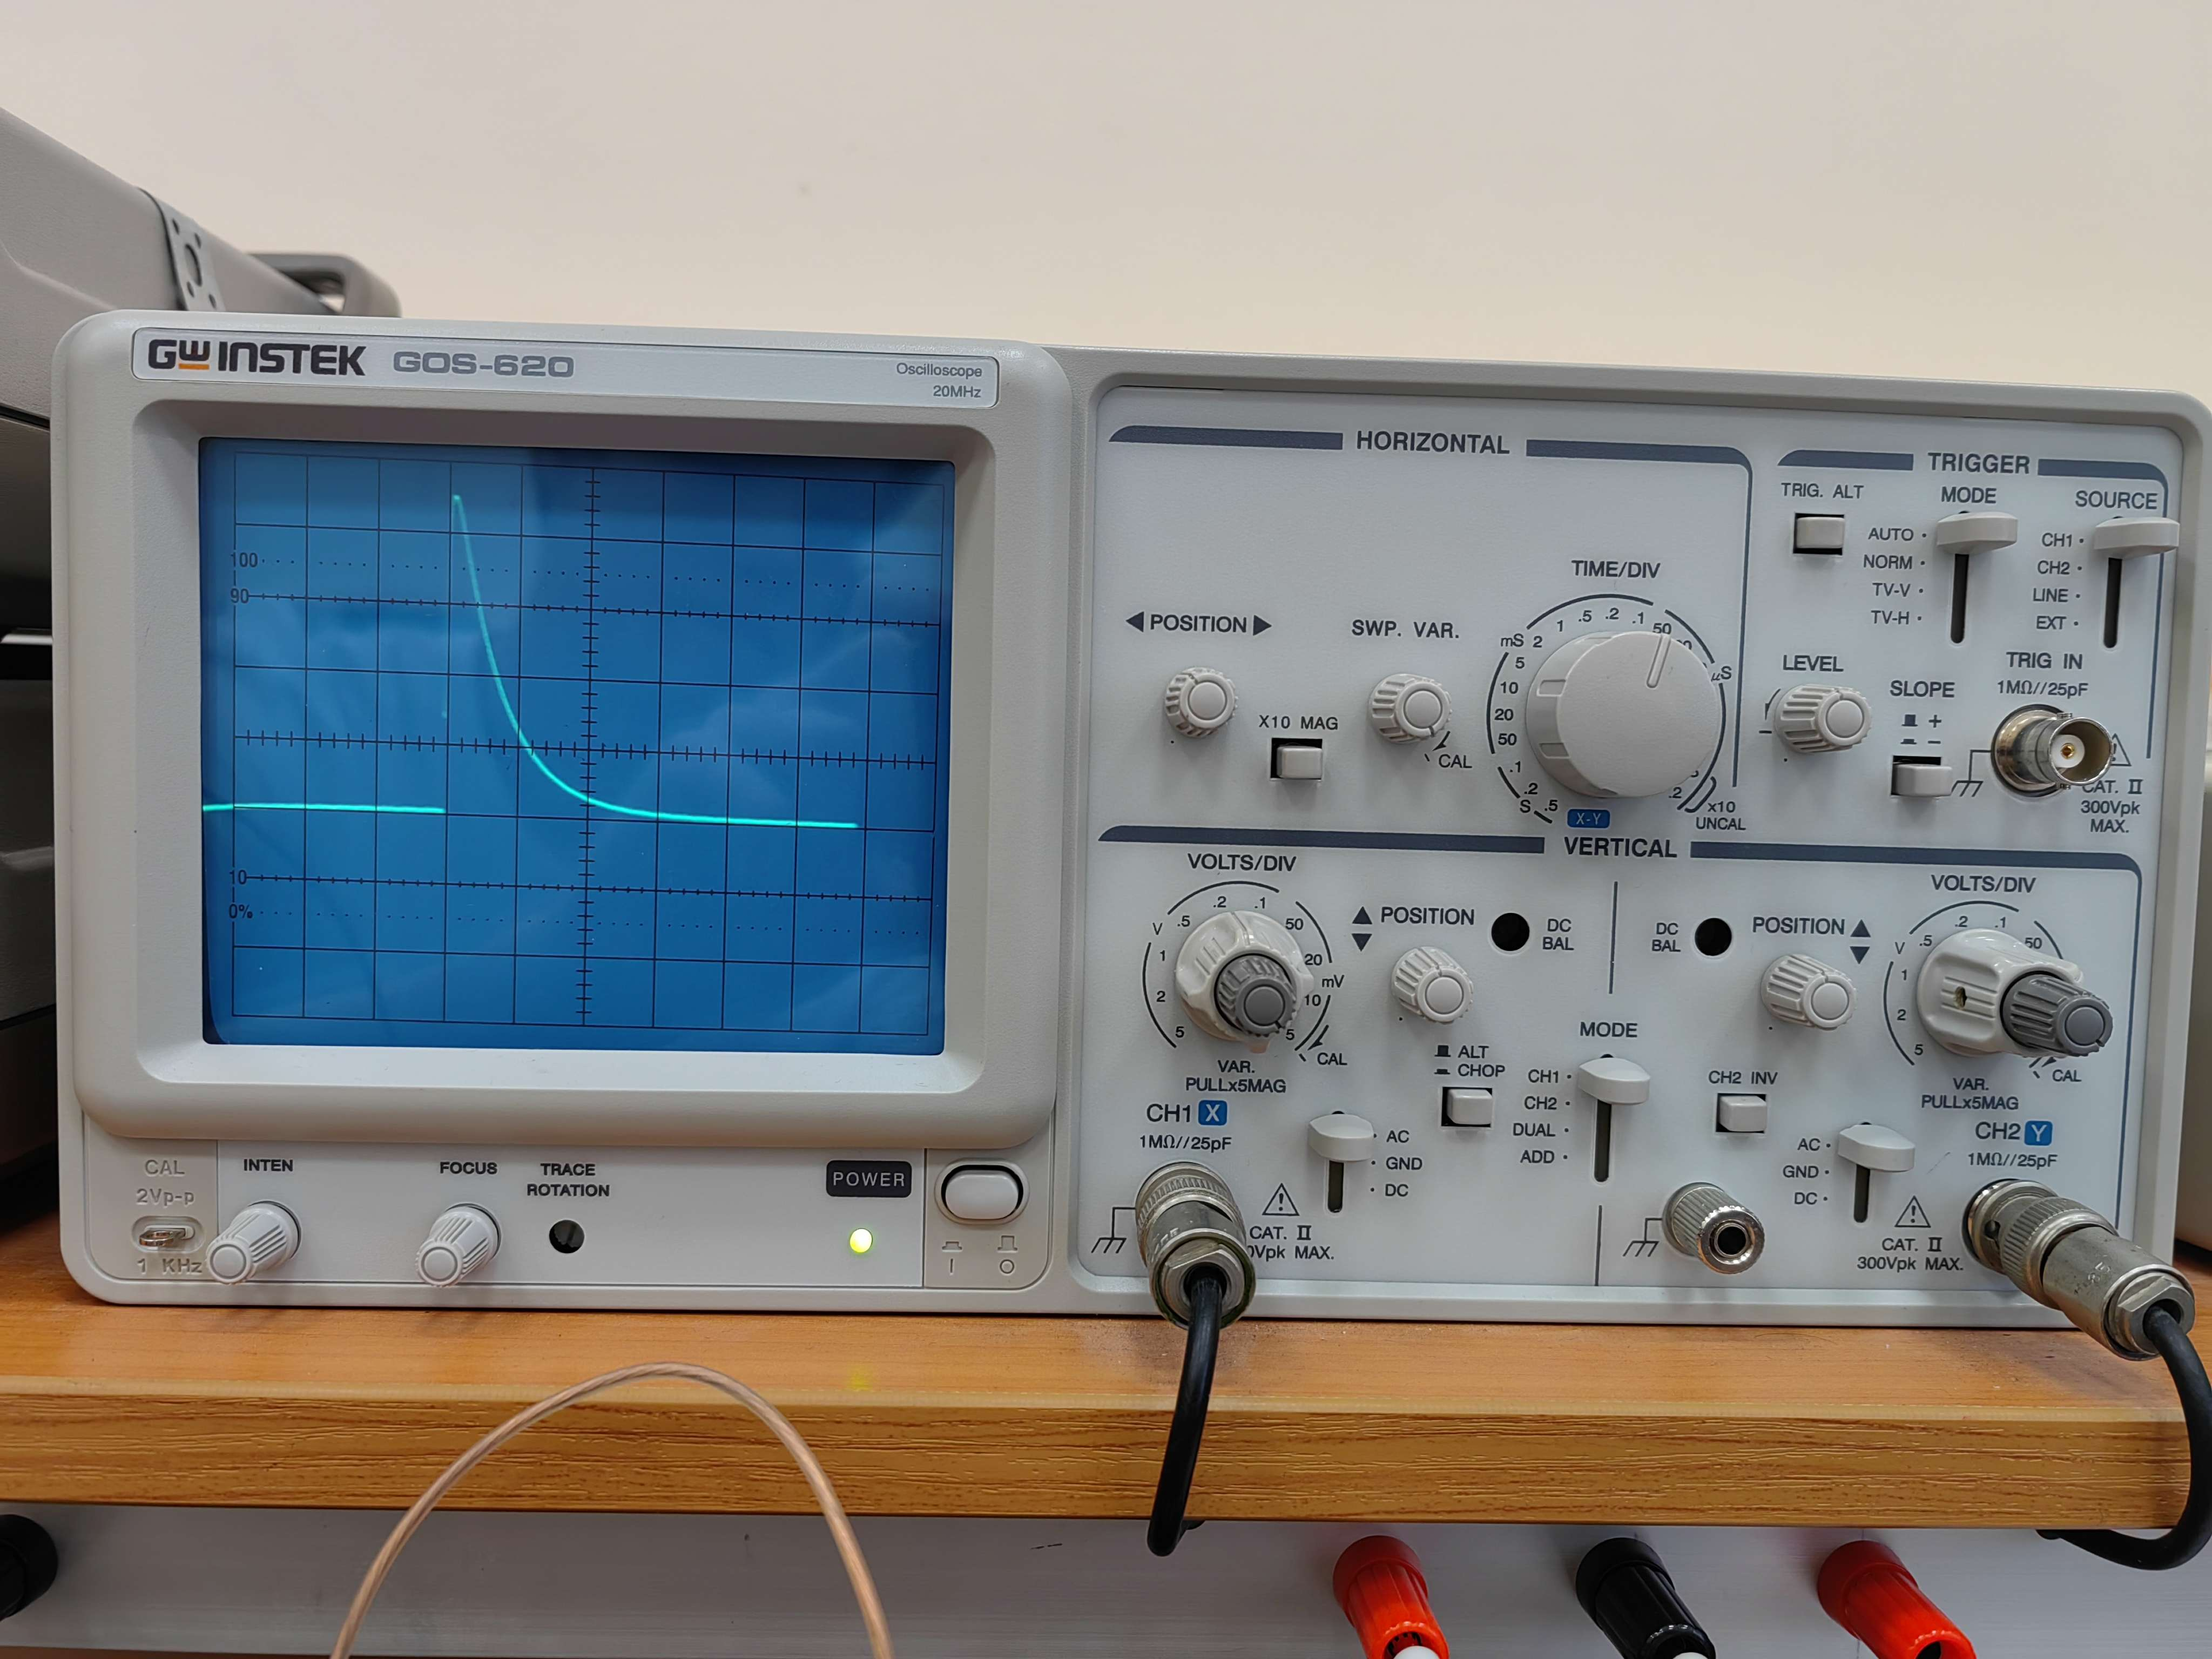
\includegraphics[width=1\textwidth]{graph3.jpg}
  \label{ris:image5}
  рис. 5 - осциллограмма для опыта №2 при R = 3, масштаб $T = .1; V = .2$
\end{figure}
\newpage
\subparagraph*{Найдем собственные частоты при $R_{cr}$ = 1.8 $k\Omega$}

\[ \alpha = \frac{R_{cr}}{2L} = \frac{1.8\cdot 10^3}{2\cdot 25\cdot 10^{-3}} = 36000 \]
\[ \omega_0 = \frac{1}{\sqrt{LC}} = \frac{1}{\sqrt{25\cdot 10^{-3}\cdot 0.02\cdot 10^{-6}}} = 44721 \]
\[ \omega = \sqrt{\omega_0^2 - \alpha^2} = j \cdot 22467 \]
\[ p_{1,2} = -\alpha \pm \sqrt{\omega_0^2 - \alpha^2} = -36000 \pm j\cdot 22467 \]
\par Согласно экспериментальным данным, в цепи будет наблюдаться критический режим, т.е. режим, граничный между колебательным и периодическим. В данном случает осциллограмма будет выглядеть так
\begin{figure}[h!]
  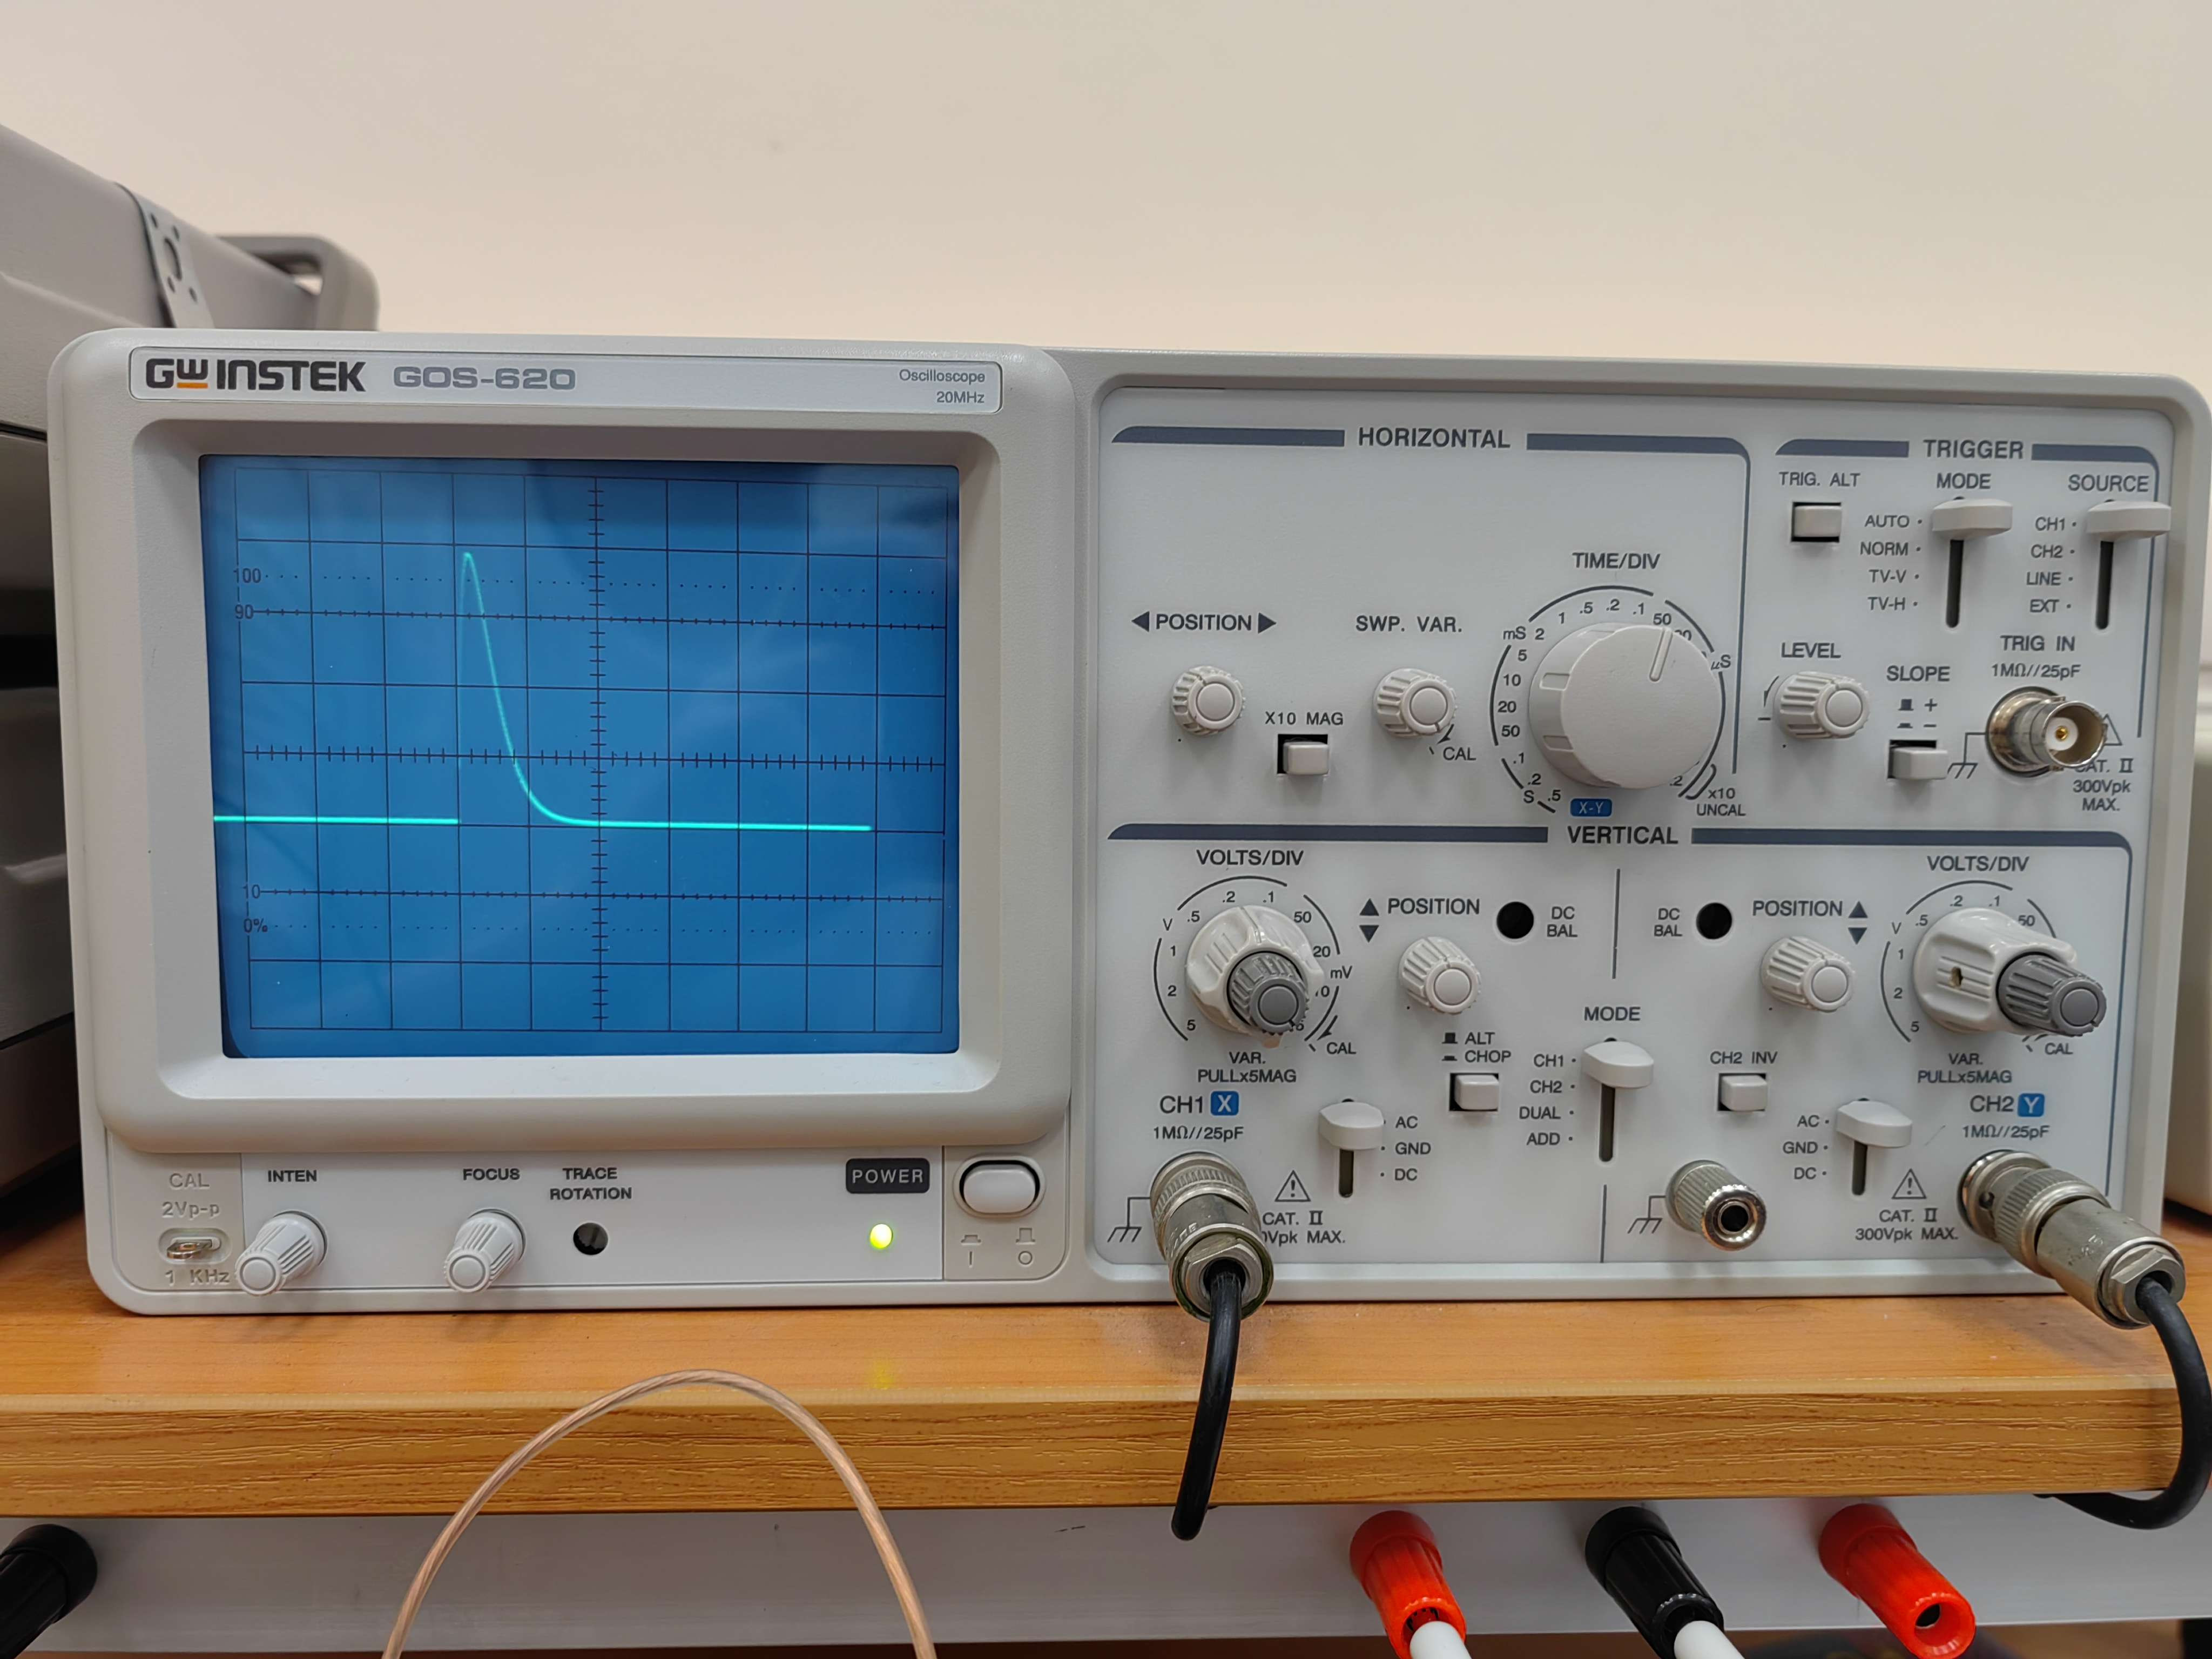
\includegraphics[width=1\textwidth]{graph4.jpg}
  \label{ris:image6}
  рис. 6 - осциллограмма для опыта №2 при R = 1.8, масштаб $T = .1; V = .2$
\end{figure}

\newpage
\subparagraph*{Найдем собственные частоты при $R$ = 0 $k\Omega$}

\[ \alpha = \frac{R_{cr}}{2L} = \frac{0\cdot 10^3}{2\cdot 25\cdot 10^{-3}} = 0 \]
\[ \omega_0 = \frac{1}{\sqrt{LC}} = \frac{1}{\sqrt{25\cdot 10^{-3}\cdot 0.02\cdot 10^{-6}}} = 44721 \]
\[ \omega = \sqrt{\omega_0^2 - \alpha^2} = j \cdot 211 \]
\[ p_{1,2} = -\alpha \pm \sqrt{\omega_0^2 - \alpha^2} = 0 \pm j\cdot 211 \]
\begin{figure}[h!]
  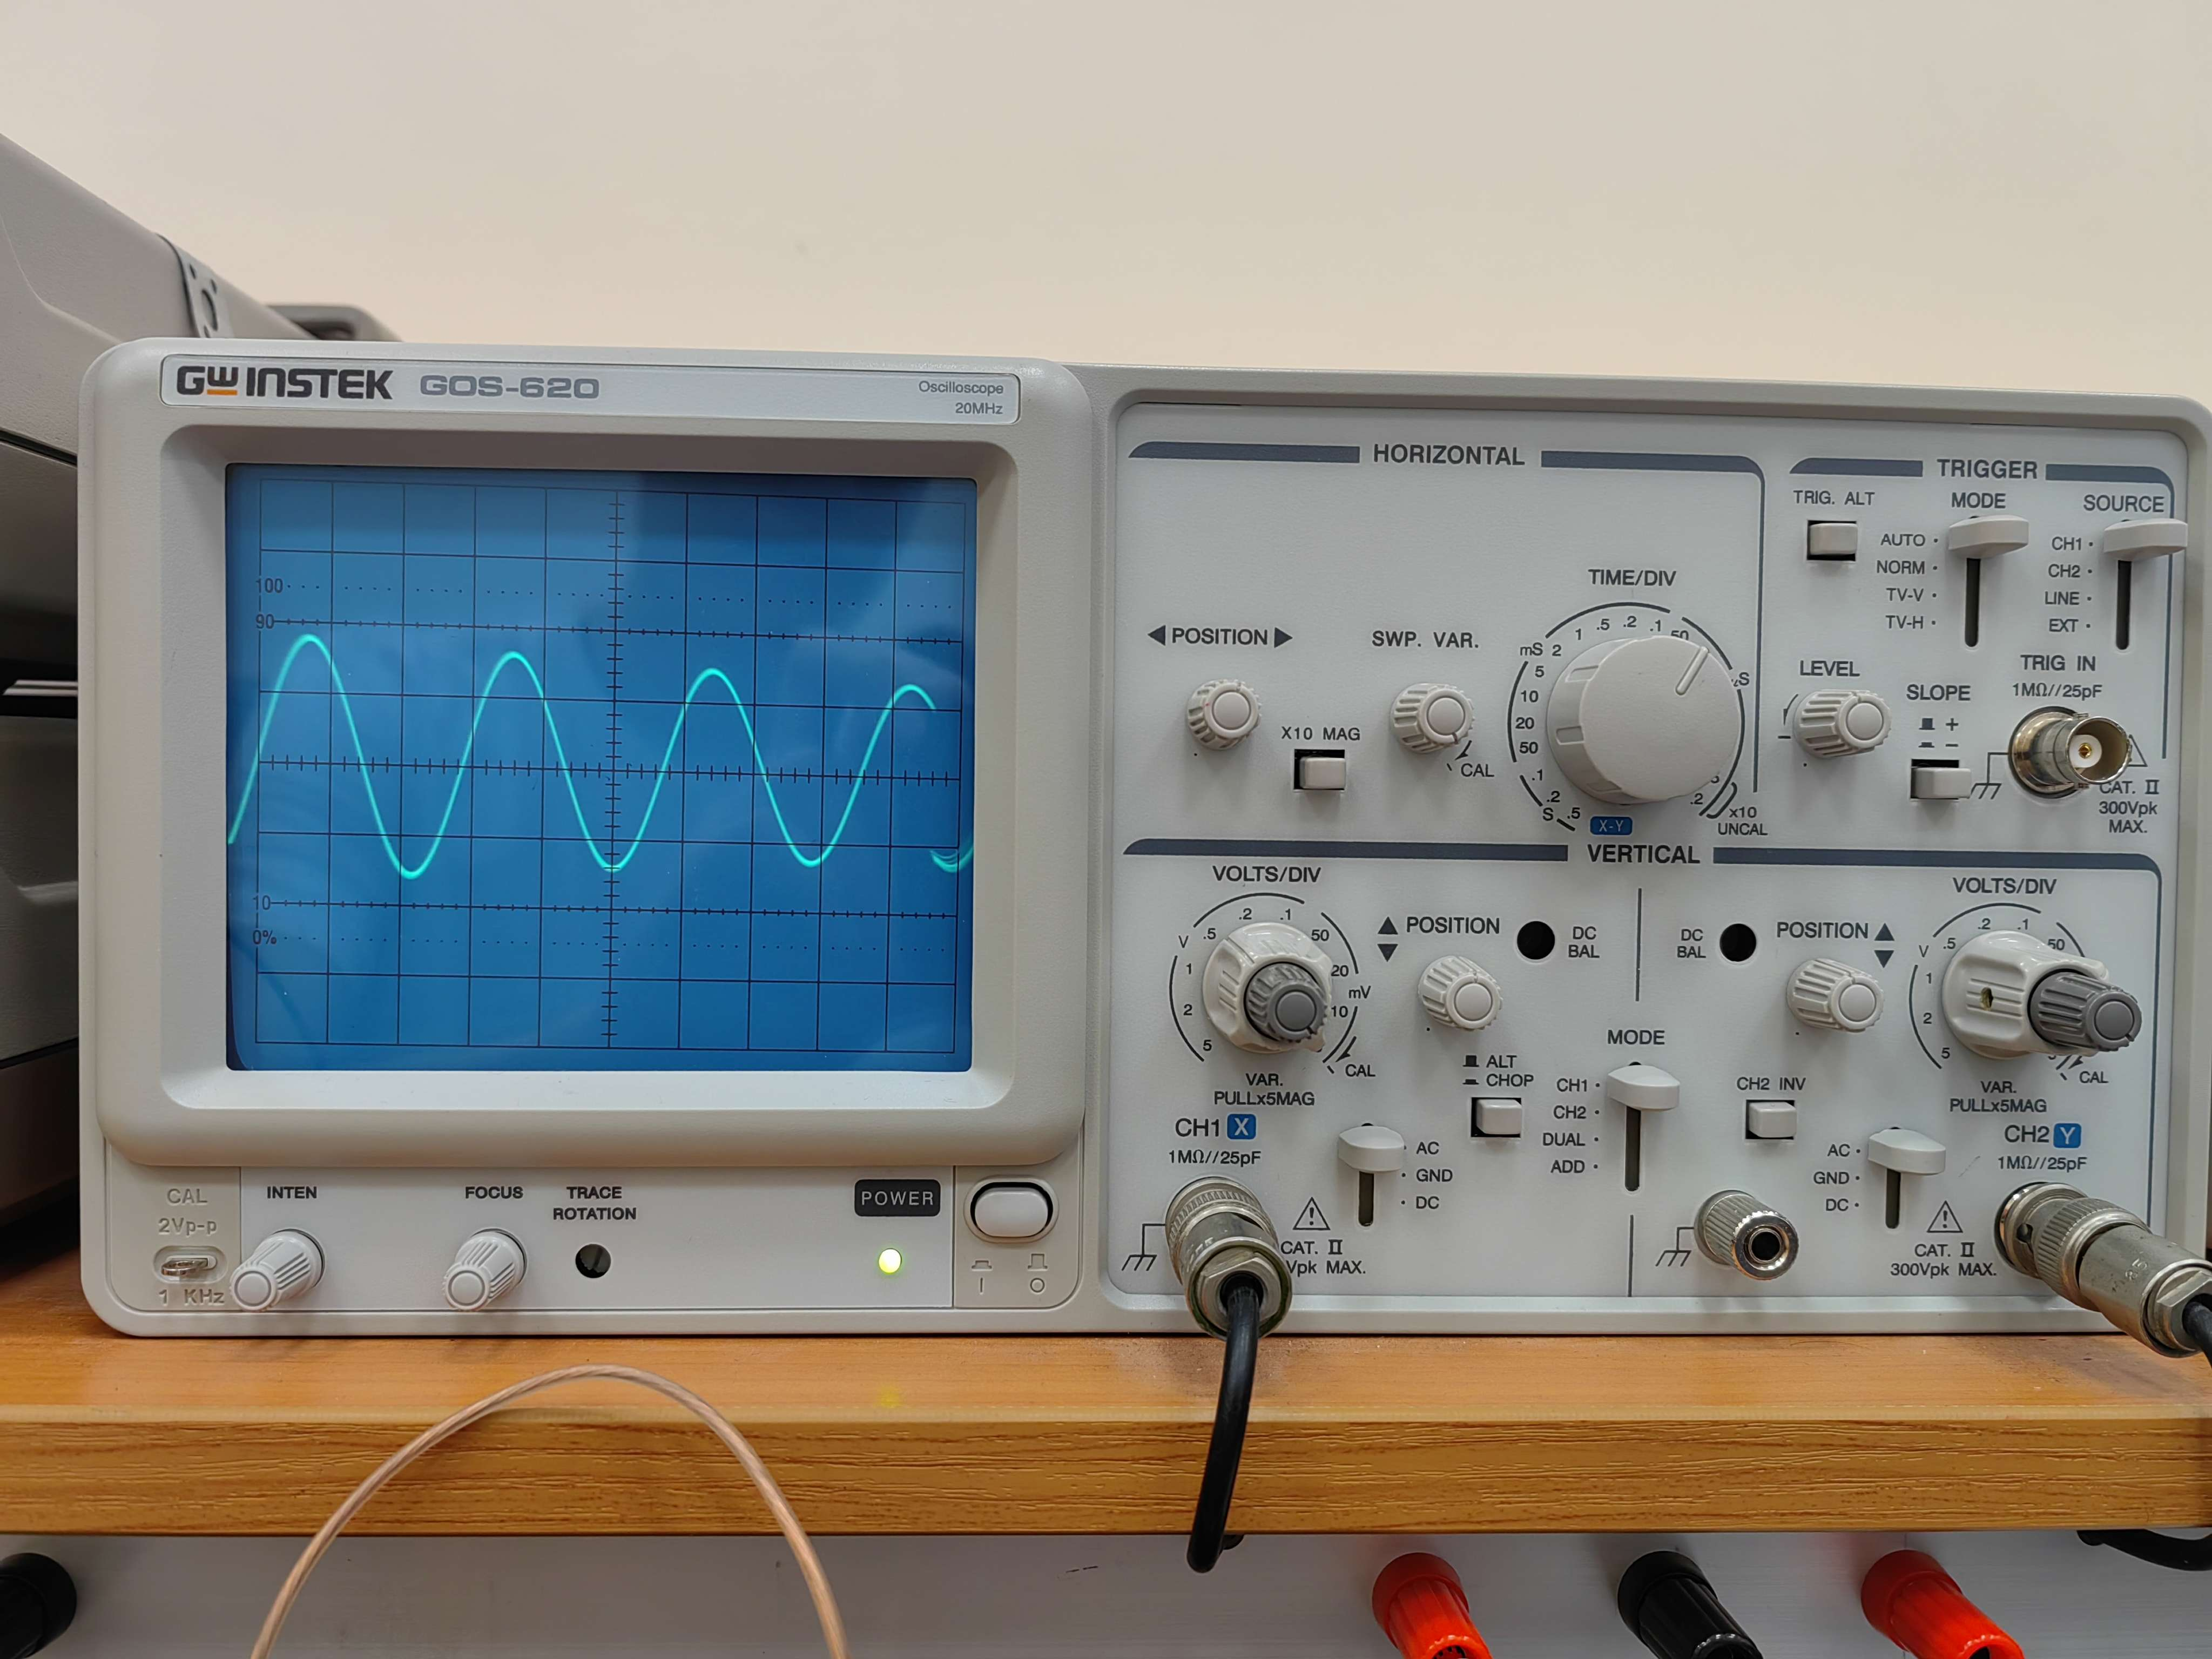
\includegraphics[width=1\textwidth]{graph5.jpg}
  \label{ris:image7}
  рис. 7 - осциллограмма для опыта №2 при R = 0, масштаб $T = 2.5\cdot 10^{-3}; V = .5$
\end{figure}

  \newpage

  \subsection*{Вопрос 3: Какими аналитическими выражениями (в общем виде) описываются процессы во всех четырех случаях? \\Графики процессов описываются выражением}
  \[ u(t) = A_1e^{-\alpha_1 t} + A_2e^{-\alpha_2 t}\] для апереодического режима
  \[ u(t) =  + A_2e^{-\alpha_2 t}\] для предельного апереодического режима(критического режима)
  \[ u(t) = Ae^{-at}\cos(\omega t + \beta)\] для колебательного режима
	\subsection*{Вопрос 4: Соответствуют ли найденные собственные частоты теоретическому расчету?}
  \subsection*{4.1: Расчет частоты цепи при $R$ = 0.5 $k\Omega$}
  \[ T = \frac{4\cdot 0.1 \, ms}{3 } \approx 0.133 \, ms \]
  \[ u_1 = 0.3 \, V \]
  \[ u_2 = 0.1 \, V \]

  \[ \alpha = \frac{\ln(u_1/u_2)}{T} = 10980 \]
  \[ \omega_0 = \frac{2 \pi}{0.133\cdot 10^{-3}} = 47242 \]

  практическое значение:
  \[ p_{1,2} = \alpha \pm j\omega = -10980 \pm j\cdot47242\]
  теоритическое значение:
  \[ p_{1,2} = \alpha \pm j\omega = -10000 \pm j\cdot43589\]
  Теоретические и практические значения очень близки друг к другу.

  \subsection*{4.2: Расчет частоты цепи при $R_{cr}$ = 1.8 $k\Omega$}
  
  практическое значение:
  \[ p_{1,2} = \alpha \pm j\omega = -40000 \pm j\cdot 20000\]
  теоритическое значение:
  \[ p_{1,2} = \alpha \pm j\omega = -40000 \pm j\cdot 23589\]
  Теоретические и практические значения очень близки друг к другу.

  \subsection*{Вопрос 5: Каковы теоретические значения собственных частот при R = 3 и соответствует ли этим значениям снятая осциллограмма? \\
   Расчет частоты цепи при $R$ = 3 $k\Omega$}
  \[ T =  0.06 \, ms \]
  \[ u_1 = 4.5 * 0.1 \, V \]
  \[ u_2 = 0.3 * 0.1 \, V \]

  \[ \alpha = \frac{\ln(u_1/u_2)}{\Delta t} = 135000\]
  \[ \omega_0 = \frac{2 \pi}{6\cdot 0.1\cdot 10^{-3}} = 10000 \]

  практическое значение:
  \[ p_{1,2} = -\alpha \pm \omega_0 = -135000 \pm 10000 \]
  \[p_1 = -125000\]
  \[ p_2 = -145000\]
  теоритическое значение:
  \[ p_{1,2} = -\alpha \pm j\omega = -60000 \pm 40000\]
  \[ p_1 = -100000 \]
  \[ p_2 = -20000 \]
  Теоретические и практические значения далеки друг от друга, что можно объяснить погрешностью измерений и несовершенством цепи, а также помехами.

  \subsection*{Вопрос №6:  Как соотносятся найденные значения добротности с результатами теоретического расчета по формуле? }
  \subparagraph*{Найдем добротность контура при $R$ = 0 $\Omega$}
\[ Q = \frac{L}{R} \cdot \omega_0 \longrightarrow \inf \]

\subparagraph*{Найдем добротность контура при $R$ = 0.5 $k\Omega$}
\[ Q = \frac{\pi}{\ln(\frac{u_1}{u_2})} = 2.85 \]

\subparagraph*{Найдем добротность контура при $R$ = 3 $k\Omega$}
\[ Q = \frac{\pi}{\ln(\frac{u_1}{u_2})\cdot 3} = 0.38 \]

\subparagraph*{Теоретические добротности: }
\subparagraph*{Найдем добротность контура при $R$ = 0 $\Omega$}
\[ Q = \frac{L}{R} \cdot \omega_0 \longrightarrow \inf \]

\subparagraph*{Найдем добротность контура при $R$ = 0.5 $k\Omega$}
\[ Q = \frac{L}{R} \cdot \omega_0 = \frac{0.025}{500}\cdot 44721 = 2.24 \]

\subparagraph*{Найдем добротность контура при $R$ = 1.8 $k\Omega$}
\[ Q = \frac{L}{R} \cdot \omega_0 = \frac{0.025}{1800}\cdot 44721 = 0.62 \]

\subparagraph*{Найдем добротность контура при $R$ = 3 $k\Omega$}
\[ Q = \frac{L}{R} \cdot \omega_0 = \frac{0.025}{3000}\cdot 44721 = 0.37 \]
  
Полученные значения достаточно близки к теоретическим.

\end{flushleft}
\newpage

\section*{Вывод}
В ходе работы было проведено исследование свободных процессов в цепи первого и второго порядка. Был произведён расчёт собственных частот цепи, а также добротность при помощи теоретического и экспериментального подхода к измерениям. В результате полученных расчётов и измерений теоретические данные кроме случая ($R = 3 \, k\Omega$) совпали с практическими.

\end{document}
